
\def\tableconfiguration{ | p{4cm} | p{2.3cm} | p{4cm} | p{4cm} | }

\index{itk::Transform|textbf}

In the toolkit, \code{itk::Transform} objects encapsulate the mapping of points
and vectors from an input space to an output space.  If a transform is
invertible, back transform methods are also provided.  Currently, ITK provides
a variety of transforms from simple translation, rotation and scaling to
general affine and kernel transforms.  Note that, although in this section we
discuss transforms in the context of registration, transforms are general and
can be used for other applications. Some of the commonly used transforms will
be discussed in detail later. Let's introduce first the objects used in ITK for
for representing basic spatial concepts.

\subsection{Geometrical Representation}
\label{sec:GeometricalObjects}

\begin{figure}
\center
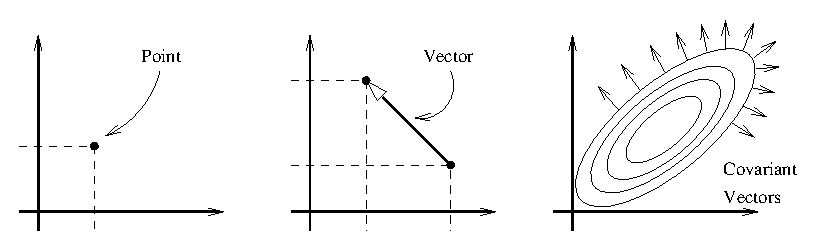
\includegraphics[width=14cm]{GeometricalObjects.eps}
\caption{Geometrical representation objects in ITK.}
\label{fig:GeometricalObjects}
\end{figure}
 
Insight implements a consitent geometric representation of the space. The
characteristics of classes involved in this representation are summarized in
the following table.

\index{itk::Point!Concept}
\index{itk::Vector!Concept}
\index{itk::CovariantVector!Concept}

\begin{center}
\begin{tabular}{ | p{4cm} | p{ 11cm } | }
\hline
\textbf{Class} &
\textbf{Geometrical concept} \\
\hline\hline
\code{itk::Point} & 
Position in space. In a $N$-Dimensional space it is represented by an array of
$N$ numbers associated with space coordinates. \\
\hline
\code{itk::Vector} & 
Relative position between two points. In a $N$-Dimensional space is represented
by an array of $N$-numbers each one associated with the distance along a
coordinate axis. Vectors do not have a position in space.\\
\hline
\code{itk::CovariantVector} & Orthogonal direction to a $(N-1)$-dimensional
manifold in space. For example, in $3D$ it corresponds to the vector orthogonal
to a surface. This is the appropriate class for representing gradients of
functions. Covariant vectors do not have a position in space.\\
\hline
\end{tabular}
\end{center}

Additional uses of the \code{Point}, \code{Vector} and \code{CovariantVector}
classes have been discussed in Chapter \ref{sec:DataRepresentation}.  Each one
of these classes behaves differently under spatial transformations. It is
henceforth quite important to keep their distinction clear. Figure
\ref{fig:GeometricalObjects} illustrates schematically the differences between
these concepts.


\index{itk::Transform!TransformPoint()}
\index{itk::Transform!TransformVector()}
\index{itk::Transform!TransformCovariantVector()}

\code{itk::Transform} classes provide different methods for mapping each one of
the basic space-representation objects.  Points, vectors and covariant vectors
are transformed using the methods \code{TransformPoint()},
\code{TransformVector()} and \code{TransformCovariantVector()} respectively.

\subsection{Transform General Properties}
\label{sec:TransformGeneralProperties}

\index{itk::Transform!SetParameters()}
Typically each transform class have several methods for setting its parameters.
For example, \code{Euler2DTransform} provide methods for separately setting the
offset, the angle, and the entire rotation matrix.  However, for use in the
registration framework, the parameters must also be represented by a flat
\code{Array<double>} to allow communication with generic optimizers. In the
case of \code{Euler2DTransform}, the transform is also defined by three
doubles: the first representing the angle and the last two the offset. The flat
array of parameters is defined using \code{SetParameters()}. A description of
the parameters and their ordering is documented in the following sections.
 
In the context of registration, the transform parameters define the search
space for optimizers. That is, the goal of the optimization is to find the set
of parameters defining a transform that results in the best possible value of
an image metric. The more parameters a transform has, the longer its
computational time will be when used in a registration method since the
dimension of the search space will be equal to the number of transform
parameters.

\index{itk::Transform!GetJacobian()}

Another requirement that the registration framework imposes on the transform
classes is the computation of their Jacobians. In general, metrics require the
knowledge of the Jacobian in order to compute the metric derivatives.  The
Jacobian is a matrix whose element are the partial derivatives of the output
point with respect to the array of parameters that defines the
transform\footnote{Note that the term \emph{Jacobian} is also commonly used for
the matrix representing the derivatives of output point coordinates with
respect to input point coordinates. Sometimes the term is loosely used to refer
to the determinant of such matrix.}:

\begin{equation}
J=\left[ \begin{array}{cccc}
\frac{\partial x_{1}}{\partial p_{1}} & 
\frac{\partial x_{1}}{\partial p_{2}} & 
\cdots  & \frac{\partial x_{1}}{\partial p_{m}}\\
\frac{\partial x_{2}}{\partial p_{1}} & 
\frac{\partial x_{2}}{\partial p_{2}} & 
\cdots  & \frac{\partial x_{2}}{\partial p_{m}}\\
\vdots  & \vdots  & \ddots  & \vdots \\
\frac{\partial x_{n}}{\partial p_{1}} & 
\frac{\partial x_{n}}{\partial p_{2}} & 
\cdots  & \frac{\partial x_{n}}{\partial p_{m}}
\end{array}\right]
\end{equation}

Where $\{p_i\}$ are the transform parameters and $\{x_i\}$ are the coordinates
of the output point.  Within this framework, the Jacobian is represented by a
\code{Array2D<double>} and is obtained from the transform by method
\code{GetJacobian()}. The Jacobian can be interpreted as a matrix that
indicates for a point in the input space how much its mapping on the output
space will change as a response to a small variation in one of the transform
parameters. Note the the values of the Jacobian matrix depend on the point in
the input space. So actually the Jacobian can be noted as $J(\bf{X})$. The use
of transform Jacobians allows to compute metric derivatives in a very efficient
way. When Jacobians are not available, metrics derivatives have to be computed
using finite difference at a price of $2M$ evaluations of the metric value,
where $M$ is the number of transform parameters.

The following sections describe the main characteristics of the transform
classes availables in ITK.

\subsection{Identity Transform}
\label{sec:IdentityTransform}

\begin{center}
\begin{tabular}{\tableconfiguration}
\hline
\textbf{Behavior} &
\textbf{Number of parameters} &
\textbf{Parameter Ordering} &
\textbf{Restrictions} \\
\hline\hline
Maps every point to itself, every vector to itself and every covariant vector to itself.  & 
0 &
  &  
Only defined when the input and output space has the same number of dimensions. \\
\hline
\end{tabular}
\end{center}

The identity transform is mainly used for debugging purposes. It is a mechanism
to provide a transform to methods that require it but yet have the certainty
that the transform will have no effect whatsoever in the outcome of the
process. It is just a \code{NULL} operation.


\subsection{Translation Transform}
\label{sec:TranslationTransform}

\begin{center}
\begin{tabular}{\tableconfiguration}
\hline
\textbf{Behavior} &
\textbf{Number of parameters} &
\textbf{Parameter Ordering} &
\textbf{Restrictions} \\
\hline\hline
Represents a simple translation of points in the input space
and has no effect on vectors or covariant vectors. &
Same as the input space dimension. &
The $i$-th parameter represents the translation in the $i$-th dimension. &
Only defined when the input and output space has the same number of dimensions. \\
\hline
\end{tabular}
\end{center}


The translation transform is probably the simplest yet useful transformation.
It maps all points in space by adding a constant values to their coordinates.
Vector and Covariant vectors remain unchanged under this transformation since
they are not associated to a position in space. Translation is the best
transform to start a registration method. Before attempting to solve for
rotations or scaling  it is important to overlap the anatomical objects in both
images as much as possible. This is done by resolving the translation
miss-registration between the images. Translations have also the advantages of
being a fast transform and having parameters that are easy to interpret.



\subsection{Scale Transform}
\label{sec:ScaleTransform}

\begin{center}
\begin{tabular}{\tableconfiguration}
\hline
\textbf{Behavior} &
\textbf{Number of parameters} &
\textbf{Parameter Ordering} &
\textbf{Restrictions} \\
\hline\hline
Points are transformed by multiplying each one of their coordinates by the
corresponding scale factor for this dimension.  Vector are transformed as
points.  Covariant vectors are transformed by \emph{dividing} their components
by the scale factor of the corresponding dimension.  &
Same as the input space dimension. &
The $i$-th parameter represents the scaling in the $i$-th dimension. &
Only defined when the input and output space has the same number of dimensions. \\
\hline
\end{tabular}
\end{center}

This transform represents a simple scaling of the vector space.  Different
scaling factors can be applied along each dimension. Points are transformed by
multiplying each one of their coordinates by the  corresponding scale factor
for this dimension.  Vector are transformed in the same way as points.
Covariant vectors, on the other hand, are transformed differently since
anisotropic scaling does not preserve angles. Covariant vectors are transformed
by \emph{dividing} their components by the scale factor of the corresponding
dimension. In this way, if a covariant vector was orthogonal to a vector, this
orthogonality will be preserved after the transformation. The following
equations summarize the effect of the transform on the basic geometric objects.

\begin{equation}
\begin{array}{lccccccc}
\mbox{Point }          & \bf{P'} &  =  & T(\bf{P})  & : & \bf{P'}_i &  = & \bf{P}_i \cdot S_i \\
\mbox{Vector}          & \bf{V'} &  =  & T(\bf{V})  & : & \bf{V'}_i &  = & \bf{V}_i \cdot S_i \\
\mbox{CovariantVector} & \bf{C'} &  =  & T(\bf{C})  & : & \bf{C'}_i &  = & \bf{C}_i /     S_i \\
\end{array}
\end{equation}

where $\bf{P}_i$, $\bf{V}_i$ and $\bf{C}_i$ are the point, vector and covariant
vector $i$-th components while $S_i$ is the scaling factor along dimension
$i$.  

Scaling is an apparently simple transformation but actually has a number of
issues to keep in mind in particular when it is used with different factors
along every dimension. It has subtle effects in things like computing image
derivatives. Since derivatives are represented by covariant vectors their
values are modified in a particular way by scaling transforms.

One of the difficulties in managing scaling transforms in a registration
process is that typical optimizers manage the parameter space as a vector space
in which addition is the basic operation. Scaling would be treated more
naturally in the frame of a logarithmic space where additions will results in
regular multiplicative increments of the scale. Optimizers in the family of
gradient-descent will have trouble finding a step-length appropriate for
updating a scale since the effect of an additive increment on a scale factor
will diminish as the factor grows. In other words, a scale factor variation of
$(1.0+ \epsilon)$ is quite different from a scale variation of $(5.0+\epsilon)$.

Registrations involving scale transforms require carefully monitoring of the
optimizer parameters in order to keep it running at an interesting yet stable
pace. Note that some of the transforms discussed in following sections, for
example the AffineTransform, have hidden scaling parameters and are henceforth
subject to the same vulnerabilities of the ScaleTransform.

In cases involving miss-registration with simultaneous translation, rotation
and scaling components it may be desirable to solve for these components
independently.


\subsection{Euler2DTransform}
\label{sec:Euler2DTransform}

\begin{center}
\begin{tabular}{\tableconfiguration}
\hline
\textbf{Behavior} &
\textbf{Number of parameters} &
\textbf{Parameter Ordering} &
\textbf{Restrictions} \\
\hline\hline
Represents a 2D rotation and a 2D translation. Note that the translation
component has no effect on the transformation of vectors and covariant vectors. &
3 &
The first parameter is the angle in radian and the last two parameters
are the translation in each dimension. &
Only defined for two-dimensional input and output spaces. \\
\hline
\end{tabular}
\end{center}

Euler2DTransform implements a Rigid transformation in $2D$. It is composed of a
plane rotation and a two-dimensional translation. The rotation is applied
first, followed by the translation. The difficult aspect of this transformation
is the fact that translations and rotations do not form a vector space and can
not be managed as linear independent parameters. Typical optimizers make the
loose assumption of managing the parameters as a vector space and rely on the
step-length to be small enough for this assumption to hold approximately.

In addition to the non-linearity of the parameter space, the most common
difficulty on this transform is the difference in units used for rotations and
translations. Rotations are measured in radians, hence their values are in the
range $[-\pi,\pi]$. Translations are measured in millimeters and their actual
values vary depending on the image modality being considered. In practice,
translations have values on the order of $10$ to $100$. This scale difference
between rotation and translation parameters is undesirable for gradient-descent
optimizers because they deviate the trayectories of descent making optimization
slower and more unstable. In order to compensate these differences, ITK
optimizers accept an array of scale values that are used to normalize the
parameter space.

Registrations involving angles and translations should take advantage of the
scale normalization funtionality in order to get the best performance out of
the optimizers.



\subsection{Similarity2DTransform}
\label{sec:Similarity2DTransform}

\begin{center}
\begin{tabular}{\tableconfiguration}
\hline
\textbf{Behavior} &
\textbf{Number of parameters} &
\textbf{Parameter Ordering} &
\textbf{Restrictions} \\
\hline\hline
Represents a 2D rotation, homogeneous scaling and a 2D translation. Note that
the translation component has no effect on the transformation of vectors and
covariant vectors. & 
4 &
The first parameter is the angle in radian, the second the scaling factor for
all dimensions and the last two parameters are the translation in each
dimension. & 
Only defined for two-dimensional input and output spaces. \\
\hline
\end{tabular}
\end{center}

A similarity transform preserves angles. It can be seen as a rigid transform
plus an isotropic scaling factor. The four parameters of this transformation
combine the characteristics of the \code{Scale} and \code{Euler2DTransform}
concerning the non-linearity of the parameter space and the non-uniformity of
the measure units. Gradient-descent like optimizers should be used with caution
on such parameter spaces since the notion of gradient direction and step-length
are ill-defined.

A possible approach for supervising optimization in the parameter space of this
transform is to dynamically control the array of scales passed to the
optimizer. The effect produced by the parameters scaling  can be used to steer
the walk on the parameter space by giving preference to some of the parameters
over others. For example, perform some iterations updating only the rotation
angle then rebablance the array of scale factor in the optimizer and perform
another set of iterations updating only translations.


\subsection{QuaternionRigidTransform}
\label{sec:QuaternionRigidTransform}

\begin{center}
\begin{tabular}{\tableconfiguration}
\hline
\textbf{Behavior} &
\textbf{Number of parameters} &
\textbf{Parameter Ordering} &
\textbf{Restrictions} \\
\hline\hline
Represents a 3D rotation and a 3D translation. The rotation is specified as a
quaternion, defined by a vector of four numbers $\bf{q}$.  The relationship
between quaternion and rotation about vector $\bf{n}$ by angle $\theta$ is as
follows: \[ \bf{q} = (\bf{n}\sin(\theta/2), \cos(\theta/2))\] Note that if the
quaternion is not of unit length, scaling will also result. &
7 &
The first four parameters defines the quaternion and the last three parameters
the translation in each dimension. &
Only defined for three-dimensional input and output spaces. \\
\hline
\end{tabular}
\end{center}



\subsection{VersorRigid3DTransform}
\label{sec:VersorRigid3DTransform}


\begin{center}
\begin{tabular}{\tableconfiguration}
\hline
\textbf{Behavior} &
\textbf{Number of parameters} &
\textbf{Parameter Ordering} &
\textbf{Restrictions} \\
\hline\hline
Represents a 3D rotation and a 3D translation. The rotation is specified a
versor or unit quaternion, defined by a vector of three numbers.
These three numbers corresponds to the first three components of a quaternion.
The fourth component of the quaternion is derived such that the quaternion is of
unit length. &
6 &
The first three parameters defines the versor and the last three parameters the
translation in each dimension. &
Only defined for three-dimensional input and output spaces. \\
\hline
\end{tabular}
\end{center}



\subsection{AffineTransform}
\label{sec:AffineTransform}

\begin{center}
\begin{tabular}{\tableconfiguration}
\hline
\textbf{Behavior} &
\textbf{Number of parameters} &
\textbf{Parameter Ordering} &
\textbf{Restrictions} \\
\hline\hline
Represents an affine transform composed of rotation, scaling, shearing and
translation. The transform is specified by a $N \times N$ matrix and a $N
\times 1$ vector where $N$ is space dimension. &
$(N+1) \times N$ &
The first $N \times N$ parameters defines the matrix in column-major order
(where the column index varies the fastest).  The last $N$ parameters defines
the translate for each dimension. &
Only defined when the input and output space have the same dimension. \\
\hline
\end{tabular}
\end{center}





